% Created 2020-03-11 mié 17:56
% Intended LaTeX compiler: pdflatex
\documentclass[a4paper]{scrartcl}
\usepackage[utf8]{inputenc}
\usepackage[T1]{fontenc}
\usepackage{graphicx}
\usepackage{grffile}
\usepackage{longtable}
\usepackage{wrapfig}
\usepackage{rotating}
\usepackage[normalem]{ulem}
\usepackage{amsmath}
\usepackage{textcomp}
\usepackage{amssymb}
\usepackage{capt-of}
\usepackage{hyperref}
\usepackage{khpreamble}
\usepackage{pgfplots}
\usepackage{pdfpages}
\usepackage{circuitikz}
\usepgfplotslibrary{groupplots}
\usetikzlibrary{positioning}
\renewcommand*{\not}[1]{\ensuremath{\bar{#1}}}
\renewcommand*{\not}[1]{\ensuremath{\overline{#1}}}
\author{Kjartan Halvorsen}
\date{2020-03-11}
\title{System identification of the tank}
\hypersetup{
 pdfauthor={Kjartan Halvorsen},
 pdftitle={System identification of the tank},
 pdfkeywords={},
 pdfsubject={},
 pdfcreator={Emacs 26.3 (Org mode 9.3.6)}, 
 pdflang={English}}
\begin{document}

\maketitle

\section{Least squares, linear regression}
\label{sec:orgbed202b}

Consider observations from experiments below, where you have set some different values of the dependent variable  \(x\), run an experiments and observed the result \(y\).

  \begin{center}
  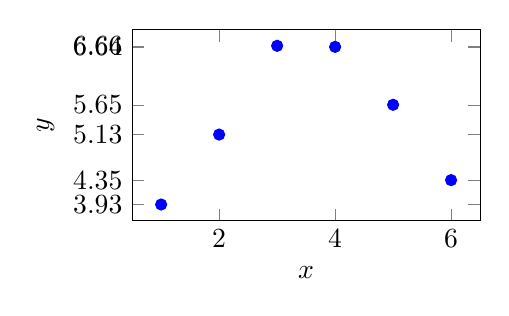
\begin{tikzpicture}
  \begin{axis}[
    width = 6cm,
    height = 4cm,
    ytick  = data,
    %    ytick = {0,4,6, 10},
    %xtick = {0,2, 4, 6, 8, 10, 12},
    %ymin = 0,
    %ymax = 10,
    ylabel = {$y$},
    xlabel = {$x$},
    ]

    \addplot[only marks, blue, domain=1:6, samples=6] { 1 + 3*x -0.4*x*x + 0.4*rand};
    
  \end{axis}
\end{tikzpicture}
\end{center}

Can you fit a suitable model to the data?

\subsection{Linear regression}
\label{sec:org21b8a5d}
Assume the model \(y = a_0x^2 + a_1x + a_2 + \epsilon\), where the residual \(\epsilon\) is the part of the observation \(y\) that cannot be explained by the model. We want to find the unknown parameters \(\theta = \begin{bmatrix} a_0 & a_1 & a_2\end{bmatrix}^T\) of the model given a set of experimental data \(\mathcal{D} = \{ (x_1, y_1),\, (x_2, y_2),\, \ldots, \, (x_N, y_N) \}\).

We can write the model as 
\begin{equation}
\begin{align} \epsilon &= y - x^2a_0 - xa_1 - a_2 = y - \phi_0(x)a_0 - \phi_1(x)a_1 - \phi_2(x)a_2 = y - \underbrace{\begin{bmatrix}  \phi_0(x) & \phi_1(x) & \phi_2(x) \end{bmatrix}}_{\text{regressors}} \begin{bmatrix} a_0\\a_1\\a_3\end{bmatrix}\\ &= y - \phi(x)^T\theta.
\end{align}
\end{equation}
The model holds for all the observations, which gives
\begin{align*}
  \epsilon_1 &= y_1 - \phi(x_1)^T\theta\\
  \epsilon_2 &= y_2 - \phi(x_2)^T\theta\\
             &\vdots\\
  \epsilon_N &= y_n - \phi(x_N)^T\theta\\
\end{align*}

Linear regression, or least-squares fitting, is defined as the optimization problem
\begin{equation}
\begin{aligned}
\text{minimize}\quad  f(\theta) &= \frac{1}{2}\sum_{i=1}^N \epsilon_i^2  = \frac{1}{2} \sum_{i=1}^N (y_i - \phi(x_i)^T\theta)(y_i - \phi(x_i)^T\theta) \\ &= \frac{1}{2} \sum_{i=1}^N \Big(y_i^2 - 2y_i\phi(x_i)^T\theta + (\phi(x_i)^T\theta)^2\Big)
\end{aligned}
\end{equation}
This optimization problem has a closed-form solution found by setting the derivative of \(f\) wrt \(\theta\) equal to zero
\[ \frac{d}{d\theta} f(\theta) = 0 \]
\[ \frac{1}{2} \sum_{i=1}^N \Big( -2y_i\phi(x_i)}^T + 2(\phi(x_i)^T\theta)\phi(x_i)^T \big)
      = \sum_{i=1}^N \Big( -y_i\phi(x_i)^T + (\theta^T\phi(x_i))\phi(x_i)^T\big) = 0 \]
which is equivalent to (by taking the transpose on both sides)
\[ \sum_{i=1}^N \Big( \phi(x_i) \phi(x_i)^T \theta - \phi(x_i) y_i\Big) = 0.\]
\[ \Big(\sum_{i=1}^N \phi(x_i) \phi(x_i)^T\Big) \theta - \sum_{i=1}^N \phi(x_i) y_i = 0.\]
\[ \Big(\sum_{i=1}^N \phi(x_i) \phi(x_i)^T\Big) \theta =  \sum_{i=1}^N \phi(x_i) y_i .\]

Defining the matrices and vectors (with some abuse of notation)
\begin{align*}
  x &= \begin{bmatrix} x_1 & x_2 & \cdots & x_N \end{bmatrix}^T\\
  y &= \begin{bmatrix} y_1 & y_2 & \cdots & y_N \end{bmatrix}^T\\
  \epsilon &= \begin{bmatrix} \epsilon_1 & \epsilon_2 & \cdots & \epsilon_N \end{bmatrix}^T\\
  \Phi(x) &= \begin{bmatrix} \phi(x_1)^T\\\phi(x_2)^T\\\vdots\\\phi(x_N)^T\end{bmatrix}\\
\end{align*}
The problem can be written 
\[
\text{minimize}\quad  f(\theta) = \frac{1}{2}\epsilon^T\epsilon = \frac{1}{2}(y -\Phi(x)\theta)^T(y-\Phi(x)\theta)\]
with solution
\[ \theta_{LS} = \Big( \Phi(x)^T\Phi(x) \Big)^{-1} \Phi(x)^T y\]

\subsection{In practice}
\label{sec:org8566269}
Given the model \(y = a_0x^2 + a_1x + a_2 + \epsilon\) and the data \(\mathcal{D} = \{ (x_1, y_1),\, (x_2, y_2),\, \ldots, \, (x_N, y_N) \}\), form the vectors and matrices

\begin{align*}
\Phi(x) &= \begin{bmatrix} x_1^2 & x_1 & 1\\x_2^2 & x_2 & 1\\\vdots & \vdots & \vdots\\x_N^2 & x_N & 1\end{bmatrix} \\
y &= \begin{bmatrix}y_1\\y_2\\\vdots\\y_N\end{bmatrix}
\end{align*}

Find the least-squares solution to 
\[ \Phi(x)\theta = y.\]

In matlab
\begin{verbatim}
x = [x1, x2, x3, x4, x5, x6]';
y = [y1, y2, y3, y4, y5, y6]';
Phi = [x.^2, x, ones(size(x))];
theta = Phi \ y
\end{verbatim}

\subsection{What about fitting the model \(y = a_0 x^{a_1}\)?}
\label{sec:orgf11b322}
Take the logarithm (assuming positive \(x\) and \(y\))
\[ y = \log a_0 + a_1\log x\]

\section{The tank model}
\label{sec:org01022a6}

\subsection{ODE}
\label{sec:orga07be0b}

\[\frac{d}{dt} p = \alpha A \sqrt{p_s - p} = a (u_v - 5) \sqrt{p_s - p}\]

\subsection{Parameter estimation}
\label{sec:org275496d}
From experiments filling the tank with different values for \(u_v\) one obtains the following table (assuming u\textsubscript{s}=1V is p=1bar)
\begin{center}
\begin{tabular}{rrrrrr}
\(p_s\) & \(u_v\) & \(p\) & \(\Delta p\) & \(\Delta t\) & \(\dot{p}\)\\
\hline
5 & 5.5 & 0 & 0.86 & 1.51 & 0.56953642\\
5 & 6 & 0 & 0.84 & 0.22 & 3.8181818\\
5 & 9 & 0 & 1.16 & 0.238 & 4.8739496\\
\end{tabular}
\end{center}

The model is 
\[ \begin{bmatrix} (u_{v_1} - 5)\sqrt{p_s - p_1} \\
                      (u_{v_2} - 5)\sqrt{p_s - p_2} \\
		      \vdots\\
		      (u_{v_N} - 5)\sqrt{p_s - p_N} \end{bmatrix} a = \begin{bmatrix} \dot{p}_1\\ \dot{p}_2\\\vdots\\ \dot{p}_N\end{bmatrix}
\]
\end{document}